\chapter{Опис система}
\section{Хардвер}
	\begin{figure}[htb!]
		\begin{center}
			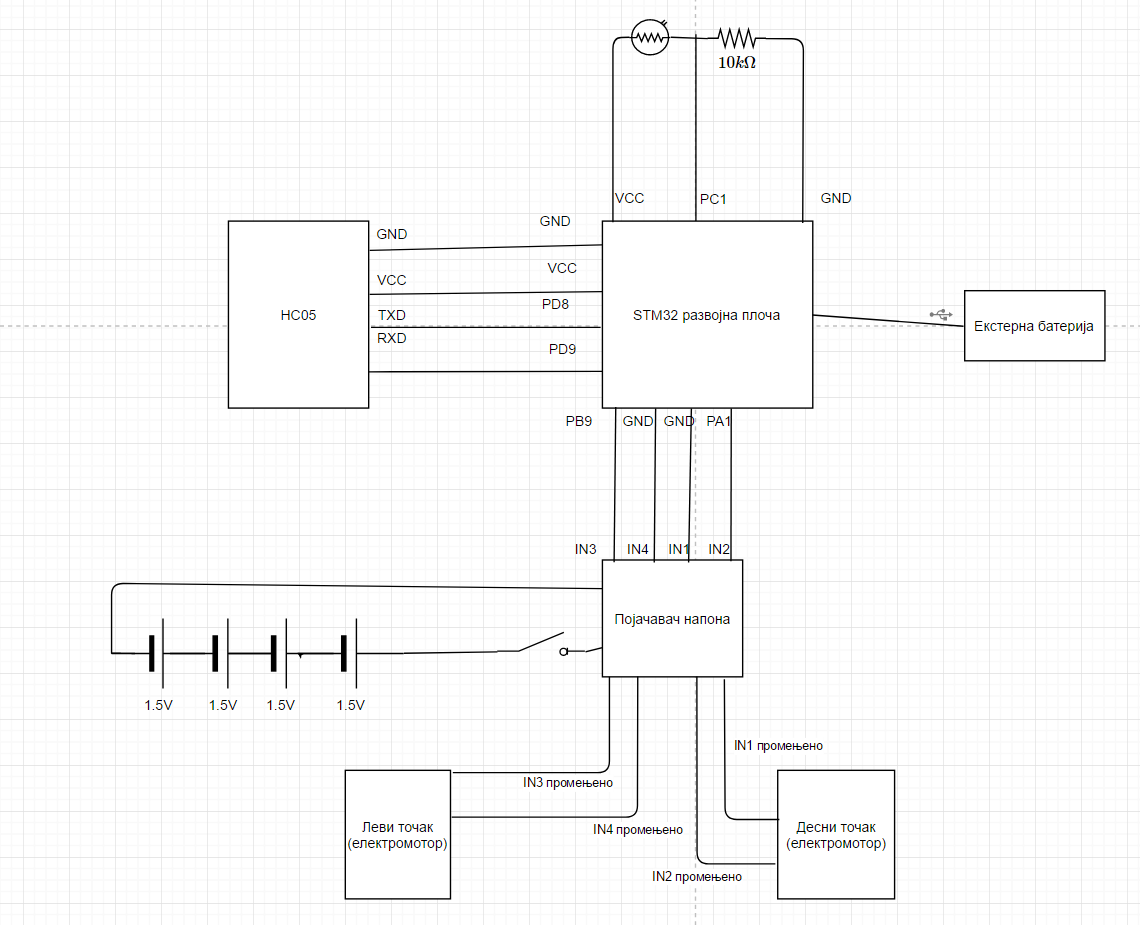
\includegraphics[scale=0.6]{pictures/Schema}
			\caption{Шема повезивања аутића}\label{fig:Schema}
		\end{center}
	\end{figure}

У наставку се налазе детаљни описи хардверских компоненти које су коришћене у изради пројекта. 

\subsection{Аутић на електромоторни погон}
У пројекту је коришћен аутић који има 2 точка који у зависности од напона окрећу се одређеним брзинама. За сваки точак постоје по два пина који примају напон, као и напајање за електромотор (објашњено касније) које појачава дате напоне да би се точкови могли да покрену. Могуће је прекинути напајање електромотора помоћу прекидача.

\subsection{Clicker2 за STM32F407VGT6}
	\begin{figure}[htb!]
		\begin{center}
			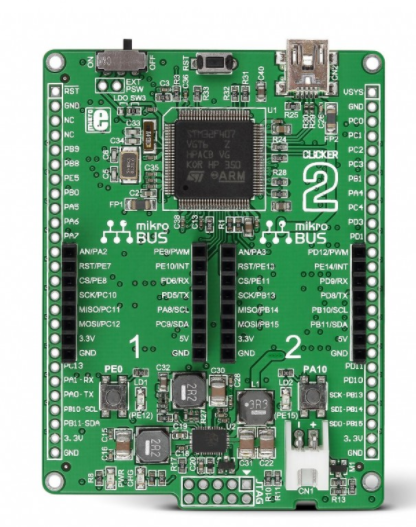
\includegraphics[scale=1]{pictures/STM32}
			\caption{STM32F407VGT6}\label{fig:STM32}
		\end{center}
	\end{figure}
Развојна плоча Clicker2 за STM32 (в. сл. \ref{fig:STM32}) је коришћена као главни модул који обрађује податке и врши управљање аутићем (преласке из одговарајућих модова у одговарајућа). На плочи се налази микроконтролер  STM32F407VGT6, 32-битни ARM Cortex M4 микроконтролер. Пропратну документацију о плочи можете наћи на \cite{STM32ST}. Из овог datasheet-а је закључено који канали могу да се користе за ADC конвертер (који је био неопходан за читање јачине светлости), као и који пинови могу да се користе за одговарајуће функционалности MCU-a (преко којих пинова може да се шаље bluetooth сигнал, преко којих може да се прима, на које може да се користи PWM MikroElekktronika библиотека ...).

\subsection{Bluetooth модул - HC-05}
	\begin{figure}[htb!]
		\begin{center}
			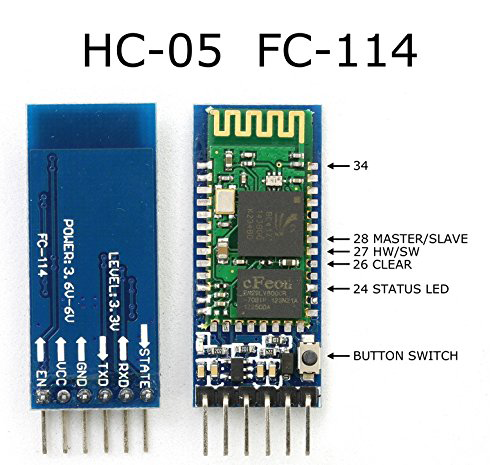
\includegraphics[scale=0.6]{pictures/Bluetooth}
			\caption{HC05} \label{fig:HC05}
		\end{center}
	\end{figure}
	Bluetooth модул HC05 (в. сл. \ref{fig:HC05}) омогућава дебаговање и тестирање функционалности аутића као што је описано у делу функционалности. Кад се упари одговарајући HC05 са уређајом који користи апликацију \cite{BluetoothTerminal}, ако је аутић у debug mode-у сваких 50ms биће слати UART протоколом подаци који су наведени у функционалностима. Комуникација је подешена на \si{9600 bps}. Модул је повезан на напајање од \si{5V} које је доведено са развојне плоче, док су његови Recieve и Transmit пинови повезани на одговарајуће пинове на развојној плочи као на шеми \ref{fig:Schema}. Datasheet који је коришћен је у линку: \cite{BluetoothModuleManual}.
	
\subsection{Фотосензор}
	\begin{figure}[htb!]
		\begin{center}
			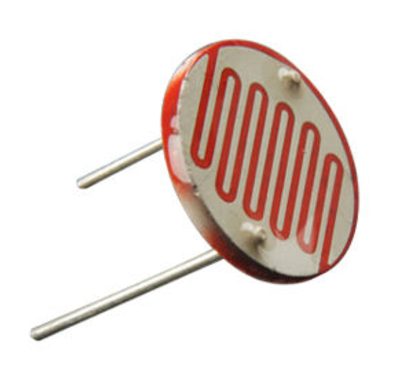
\includegraphics[scale=.2]{pictures/PhotoResistor}
			\caption{Фотоотпорник} \label{PhotoResistor}
		\end{center}
	\end{figure}		
	\begin{figure}[htb!]
		\begin{center}
			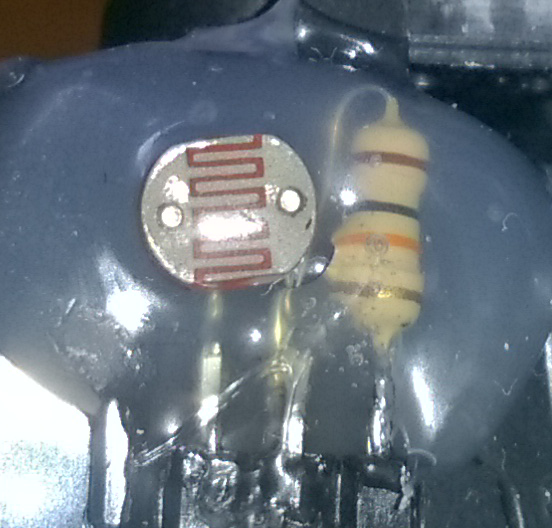
\includegraphics[scale=.15]{pictures/PhotoSensor}
			\caption{Фотосензор} \label{PhotoSensor}
		\end{center}
	\end{figure}		
	Фотоотпорник (в. сл. \ref{PhotoResistor}) повезан је на ред са отпорником oтпорности \si{10k\Omega} (као на сл. \ref{PhotoSensor}). Напајање је од \si{3,3V} је доведено на крај фотоотпорника и отпорника (GND и VCC), док је мерен напон на споју отпорника и фотосензора и добијена аналогна вредност је уз помоћ ADC конвертора са одговарајућег пина (в. шему \ref{fig:Schema}) претварана у одговарајућу дигиталну вредност и даље коришћена у развојној плочи.
	
\subsection{Напајање}
	\begin{figure}[htb!]
		\begin{center}
			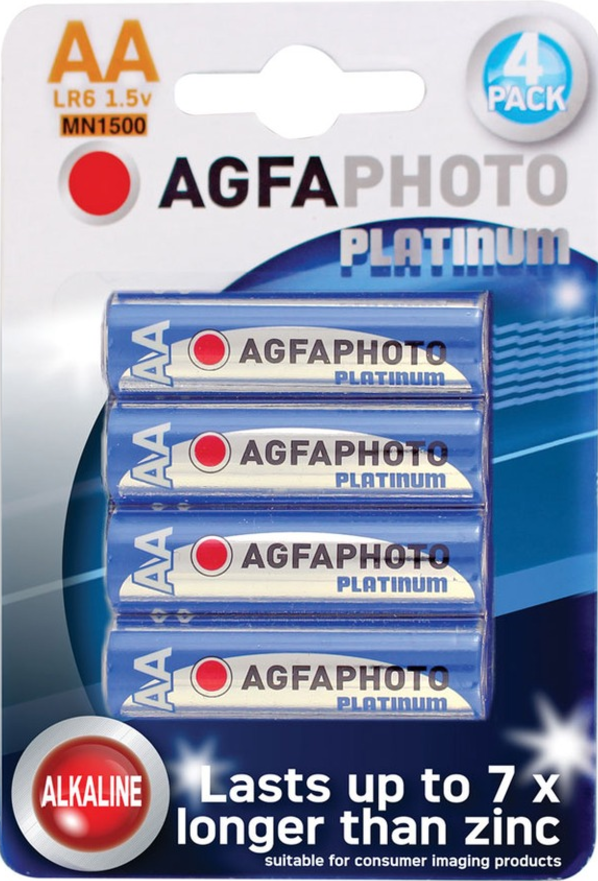
\includegraphics[scale=0.25]{pictures/AGFABattery}
			\caption{Напајање за електромотор за аутић} \label{fig:AGFA}
		\end{center}
	\end{figure}
	\begin{figure}[htb!]
		\begin{center}
			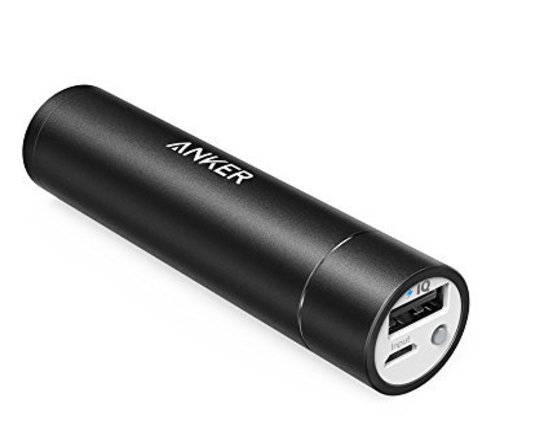
\includegraphics[scale=0.5]{pictures/ExternalBattery} 
			\caption{Напајање за развојну плочу}\label{fig:extBattery}
		\end{center}
	\end{figure}
	Пошто је за електромотор који покреће точкове било неопходно напајање од \si{6V} коришћене су 4 батерије од \si{1,5V}(в. сл. \ref{fig:AGFA}). Док на другу страну максимално напајање могуће за развојну плочу је било \si{5V}, стога је коришћена екстерна батерија (в. сл.\ref{fig:extBattery}) која преко Mini B USB-USB напаја развојну плочу. 
	\newpage
	
\section{Софтвер}
	\subsection{Programming environment}
Коришћена је microC PRO for ARM work enviroment (\cite{MICROCPRO}) који нуди могућност уређивања кода за Clicker2 развојну плочу и компајлирања истог. microC је сличан програмском језику C са тим да има одговарајуће предефинисане библиотеке (у овом пројекту PWM, UART, ADC) и макрое који олакшавају програмирање за одговарајуће MikroElektronika плоче и компоненте. За спуштање генерисаног кода у hex формату, се користи \cite{Bootloader} за Clicker2. При том развојна плоча и одговарајући рачунар, на ком је код био изгенерисан и који се спушта, морају бити повезани Mini B USB-USB конектором да би код био спуштен на развојну плочу.
	\subsection{Koд на развојној плочи}
Код се налази на: \cite{Code}. Након што се укључи уређај позивају се одговарајући сегменти кода који служе за иницијализацију одговарајућих модула аутића (bluetooth, фотосензора, pwm-а, timer-а, саме логике аутића). Након тога главни програм ставља у low power режим који чека на interrupt-ове одговарајућом ARM инструкцијом. На сваких 50ms се покреће interrupt који омогућава обављање функционалности описаних на почетку документације. 

Код је подељен у неколико фолдера:
\begin{enumerate}[1.]
	\item \textbf{util}\\
	У овом фолдеру, тј. тачније фајлу \textit{util.c} се налазе дефиниције константи које се користе у свим сегментима као и макрои који служе за експандовање пинова. Поред тога овде се налази константа која омогућава подешавање да ли је release mode или debug mode. Release mode не шаље никакве податке преко bluetooth (ради брже обраде прекида), док debug шаље (ради дебаговања и тестирања аутића). 
	\item \textbf{}
		У кореном директоријум налази се конфигурација за build-овање, као и одговарајућа улазна тачка програма (\textit{main.c}). 
	\item \textbf{bluetooth}\\
		У овом фолдеру тачније фајловима \textit{bluetooth.c} и \textit{bluetooth.h} налазе се дефиниције променљивих и функција коришћених за bluetooth размену и иницијализацију. Коришћен је UART протокол за слање. Променљиве типа \textit{string }и \textit{int } слате су преко бафера који је иницијализован на одговарајућу величину унапред.
	\item \textbf{light}\\
	У овом фолдеру, тачније у фајловима \textit{lightDetector.h} и \textit{lightDetector.c} налазе се дефиниције променљивих и функција које су коришћене за детектовање јачине светлости са улаза. Коришћена је MikroElekltronika-ина одговарајућа ADC библиотека. Она омогућава конвертовање аналогне вредности са фотоотпорника у одговарајућу дигиталну која даље може бити коришћена у програму.
	\item \textbf{pwm}\\
		У овом фолдеру, тачније у фајловима \textit{pwm.h} и \textit{pwm.c} налазе се дефиниције променљивих и функција коришћених за иницијализацију pwm библиотеке за даље коришћење у осталим сегментима кода. 
	\item \textbf{timer}\\
	У овом фолдеру, тачније у фајловима \textit{timer.h} и \textit{timer.c} налазе се дефиниције променљивих и функција коришћених за иницијализацију и обраду прекида. Константе су подешене тако да се прекид дешава сваких 50ms и при томе се обавља логика која је описана у logic фолдеру.
	\item \textbf{wheel}\\
	У овом фолдеру, тачније у фајловима \textit{wheel.h}, \textit{left.h} и \textit{left.c} односно \textit{right.h} и \textit{right.c} налазе се дефиниције променљивих, константи и функција које омогућавају кретање левог, односно десног точка, уз помоћ MikroElektronika-ине pwm библиотеке. 
	\item \textbf{logic}\\
		\begin{enumerate}[i)]
			\item \textbf{light}\\
				Логика
			\item \textbf{movement}\\
				Кретање
		\end{enumerate}


\end{enumerate}

